%!TEX root = ../dokumentation.tex

\chapter{Ergebnisverifizierung}

\section{Unit Tests}

Unit Testing ist eine Technik, die bei der Softwareentwicklung angewendet wird, um sicherzustellen, dass kleine, logisch abtrennbare Komponenten wie entworfen funktionieren und die richtigen Ergebnisse liefern. Da das manuelle Testen der Komponenten zeit- und arbeitsintensiv ist, gibt es viele Werkzeuge, um Komponententests automatisch durchzuführen. Kontinuierliche Build- und Integrationstools sorgen dafür, dass der entwickelte Code vor einem Commit fehlerfrei ist. In kollaborativer Entwicklung werden Komponenten separat entwickelt. Oft hängen bestimmte Funktionen der Software von anderen ab, wodurch Seiteneffekte schon bei kleinen Änderungen entstehen können. Durch die parallele Bereitstellung von Unit-Tests zum entwickelten Code, können negative Seiteneffekte erkannt und anschließend behoben werden \cite{Dalton2018}.

Um schnell und einfach Unit-Tests schreiben zu können, wird das Testing-Framework Mocha im Zusammenspiel mit der Assertion-Bibliothek Chai verwendet. Mocha ist ein auf Node.js laufendes JavaScript-Testing-Framework, das die Erstellung von asynchronen Tests einfach macht. Mocha-Tests werden sequentiell ausgeführt und erlauben es Fehlerzustände auf die richtigen Testfälle zuzuordnen \cite{mocha}. Chai bietet Funktionen, mit denen das Ergebnis eines bestimmten Tests mit seinem erwarteten Wert verglichen werden kann. Zudem liefert Chai eine sehr lesbare Syntax, indem es sich an der englischen Sprache orientiert \cite{chai}.

Durch eine hohe Anzahl an entwickelten Nodes im \ac{MLTDG} bieten sich optimale Komponenten für Unit-Tests an, um ihre Funktionalitäten zu testen. Im Folgenden wird beispielhaft ein Unit-Test für den $MathNode$ im \ac{MLTDG} mit Mocha und Chai erstellt.

Um einen Unit-Test mit Chai erstellen zu können, muss die Chai-Bibliothek und die zu testende Komponente importiert werden. In diesem Fall wird also der $MathNode$ importiert.

\begin{lstlisting}[caption=Unit-Test: Import,label=unit1]
import { expect } from "chai";
import MathNode from "@/nodes/MathNode";
\end{lstlisting}

Der $MathNode$ kann verschiedenste mathematische Funktionen auf maximal zwei Werte anwenden. Mit insgesamt 18 Testfällen lohnt es sich die Tests in einer Schleife zu erstellen. Dafür wird zunächst ein Array erstellt, der für jeden Testfall Name, Parameter A, Parameter B und das erwartete Ergebnis speichert.

\begin{lstlisting}[caption=Unit-Test: Testdefinition,label=unit2]
const tests = [
    ["Add", 1, 1, 2],
    ["Subtract", 1, 1, 0],
    ["Multiply", 5, 5, 25],
    ["Divide", 10, 5, 2],
    ["Sine", 2, 0, Math.sin(2)],
    ["Cosine", 2, 0, Math.cos(2)],
    ["Tangent", 2, 0, Math.tan(2)],
    ["Arcsine", 0.5, 0, Math.asin(0.5)],
    ["Arccosine", 0.5, 0, Math.acos(0.5)],
    ["Arctangent", 0.5, 0, Math.atan(0.5)],
    ["Power", 2, 2, 4],
    ["Logarithm", 4, 2, 2],
    ["Minimum", 2, 4, 2],
    ["Maximum", 2, 4, 4],
    ["Round", 4.3, 0, 4],
    ["Round", 4.7, 0, 5],
    ["Modulo", 7, 3, 1],
    ["Absolute", -1, 0, 1]
] as Array<[string, number, number, number]>;
\end{lstlisting}

Nun können die Testfälle mit Mocha implementiert werden. Mit dem  $describe$-Befehl wird den Tests eine Struktur gegeben. Der Name des zu testenden Nodes $MathNode$ ist hier völlig ausreichend. Mit einer ForEach-Schleife wird durch das Array iteriert. Der $it$-Befehl beschreibt, was genau in dem Test geprüft wird. Der $MathNode$ soll natürlich die mathematische Operation korrekt ausführen. Bei jeder Iteration wird ein neuer MathNode erstellt, die Parameter gesetzt, die zugehörige Operation ausgewählt und die Berechnung ausgelöst. Das Ergebnis kann nun mithilfe der Assertion-Bibliothek Chai einfach mit dem erwarteten Ergebnis überprüft werden. 

\begin{lstlisting}[caption=Unit-Test: Testdurchführung,label=unit3]
describe("MathNode", () => {
    tests.forEach(([op, val1, val2, expected]) => {
        it(`performs the operation '${op}' correctly`, () => {
            const n = new MathNode();
            n.getInterface("Value 1").value = val1;
            n.getInterface("Value 2").value = val2;
            const v = n.getOptionValue("Operation");
            v.selected = op;
            n.setOptionValue("Operation", v);
            n.calculate();
            expect(n.getInterface("Result").value).to.equal(expected);
        });
    });
});
\end{lstlisting}

\section{Usability-Tests}

Beim Entwickeln eines Produkts besteht die Gefahr, dass die Entwickler die Komplexität und mögliche Schwachstellen im Bereich der User Experience übersehen \cite{Witte2018}. Aus diesem Grund werden Usability-Tests durchgeführt. Diese sollen sicherstellen, dass das Produkt von den Anwendern möglichst einfach und effizient genutzt werden kann.

Laut Moser ist der Ablauf eines Usability-Tests in sechs Phasen gegliedert \cite{Moser2012}:
\begin{enumerate}
    \item Ziel und Zweck festlegen
    \item Untersuchungsdesign entwerfen
    \item Teilnehmer rekrutieren
    \item Evaluation vorbereiten
    \item Evaluation durchführen
    \item Resultate auswerten
\end{enumerate}

\subsection{Ziel und Zweck}
Ziel der Untersuchung ist es, herauszufinden, ob die Umsetzung mittels grafischer Modellierung so zugänglich ist, dass auch neue Nutzer nach dem Lesen einer kurzen Anleitung ein Modell erstellen können.

\subsection{Untersuchungsdesign entwerfen}

\subsubsection*{Vorgehen}
\begin{enumerate}
    \item Testperson liest Anleitung (ca. 3 DIN-A4 Seiten) [10 Minuten]
    \item Testperson erhält Aufgabe und hat Zeit, diese durchzulesen sowie Fragen zu stellen [5 Minuten]
    \item Testperson setzt das Modell um. Falls Fragen zur Aufgabe aufkommen, werden diese direkt vom Versuchsleiter beantwortet. Bei Fragen zur Applikation wird die Testperson ermuntert, die Antwort selber herauszufinden (zum Beispiel mit der Anleitung oder durch Experimentieren); sollte die Testperson nicht innerhalb einer angemessenen Zeitspanne auf die Antwort kommen, so wird der Versuchsleiter Hinweise geben. Der Versuch wird nicht abgebrochen, auch wenn die Testperson mehr Zeit benötigt. [30 Minuten]
    \item Befragung der Testperson durch Versuchsleiter bezüglich Benutzererlebnisses während des Tests. Außerdem wird die Testperson ermutigt, Kritik bezüglich der Bedienbarkeit zu äußern. [5 Minuten]
\end{enumerate}

\subsubsection*{Umgebung}
Die Versuche werden auf den Rechnern der Versuchsteilnehmer durchgeführt, um den Versuchspersonen eine vertraute Umgebung zu bieten. Während des gesamten Tests ist ein Versuchsleiter verfügbar, der Zugriff auf den Desktop des Versuchsteilnehmers hat und verbal mit dem Versuchsteilnehmer kommunizieren kann. Anleitung und Aufgabe werden den Versuchsteilnehmern digital zur Verfügung gestellt.

\subsection{Teilnehmer rekrutieren}

Moser empfiehlt für qualitative Tests etwa 5-10 Teilnehmer zu rekrutieren \cite{Moser2012}. Aufgrund der im Versuchsziel formulierten Anforderung werden Personen ausgewählt, die keine Vorerfahrung mit der Applikation haben.

In diesem Fall konnten 4 Teilnehmer rekrutiert werden. Alle Teilnehmer waren zwischen 20 und 60 Jahre alt und hatten zumindest grundlegende Programmierkenntnisse.

\subsection{Evaluation vorbereiten}

Die Versuchspersonen testen eine Beta-Version der Applikation vom 11. April 2019. Diese erreichen sie über ihren Browser unter eine vorgegebenen URL. Es wird vom Versuchsleiter sichergestellt, dass die Versuchspersonen Google Chrome mit Version 72 oder neuer benutzen, da die Applikation für diesen Browser optimiert ist.

Zuerst erhalten die Versuchspersonen eine Anleitung für den \ac{MLTDG}. Die Anleitung ist im Anhang A (S. \pageref{apx:manual}) zu finden.

Anschließend erhalten die Versuchspersonen folgende Aufgabe:

\begin{quote}
    
    Erstellen Sie mit dem \textit{Machine Learning Training Data Generator} eine CSV-Datei. Diese soll 1000 Datensätze enthalten. Die Datensätze sollen einen Wohnungsmarkt modellieren. Jeder Datensatz stellt dabei eine Wohnung dar, die auf dem Markt verkauft wird. Jede Wohnung hat folgende Eigenschaften (Spalten): \textbf{Fläche} (in $m^2$), \textbf{Räume}, \textbf{Garage} (true/false) und \textbf{Preis} (in Euro).

    Die Eigenschaften sind folgendermaßen zu modellieren:
    \begin{itemize}
        \item Eine Wohnung hat mit einer 50 prozentigen Chance eine \textbf{Garage}.
        \item Die \textbf{Fläche} der Wohnungen entspricht einer Normalverteilung mit dem Mittelwert $\mu = 130$ und der Standardabweichung $\sigma = 40$. Sollte bei der Fläche ein Wert $< 20$ herauskommen, ist der Datensatz ungültig und soll nicht in die Ausgabedatei übernommen werden.
        \item Die Anzahl der \textbf{Räume} ist abhängig von der Fläche. Dabei gilt folgender Zusammenhang: $\textrm{Räume} = \textrm{Fläche} / 40$.
        \item Der Preis ist abhängig von den drei vorher beschriebenen Faktoren. Dabei gilt folgender Zusammenhang:
        
        $\textrm{Preis} = 2500 \cdot \textrm{Fläche} + 250 \cdot \textrm{Räume}$.
        
        Wenn eine Garage zu der Wohnung gehört, steigert diese den Preis um $20000$ Euro. Da nicht jeder Verkäufer den Preis nach dieser Formel festlegt, kann eine prozentuale Abweichung von $\pm 5\%$ angenommen werden.
    \end{itemize}

    Das ganze Projekt soll zusätzlich in einer Datei lokal abgespeichert werden, um es zu einem späteren Zeitpunkt wieder öffnen zu können.

\end{quote}

Es werden folgende Merkmale untersucht:
\begin{itemize}
    \item Zeit, die für das Lösen der Aufgabe benötigt wird
    \item Zufriedenheit der Versuchspersonen bezüglich Usability
    \item Häufigkeit der Inanspruchnahme von Hilfe des Versuchsleiters
    \item Unerwartete Schwierigkeiten der Versuchspersonen bei der Durchführung eines konkreten Teils der Aufgabe
\end{itemize}

\subsection{Evaluation durchführen}
Die Evaluation wurde entweder persönlich durchgeführt, das heißt der Versuchsleiter war vor Ort, oder über ein Remote Desktop Tool in Verbindung mit einem Kommunikationstool. Somit konnte der Versuchsleiter in allen Fällen den Bildschirm der Teilnehmer sehen und mit diesen über Sprache kommunizieren.

\begin{figure}[H]
    \centering
    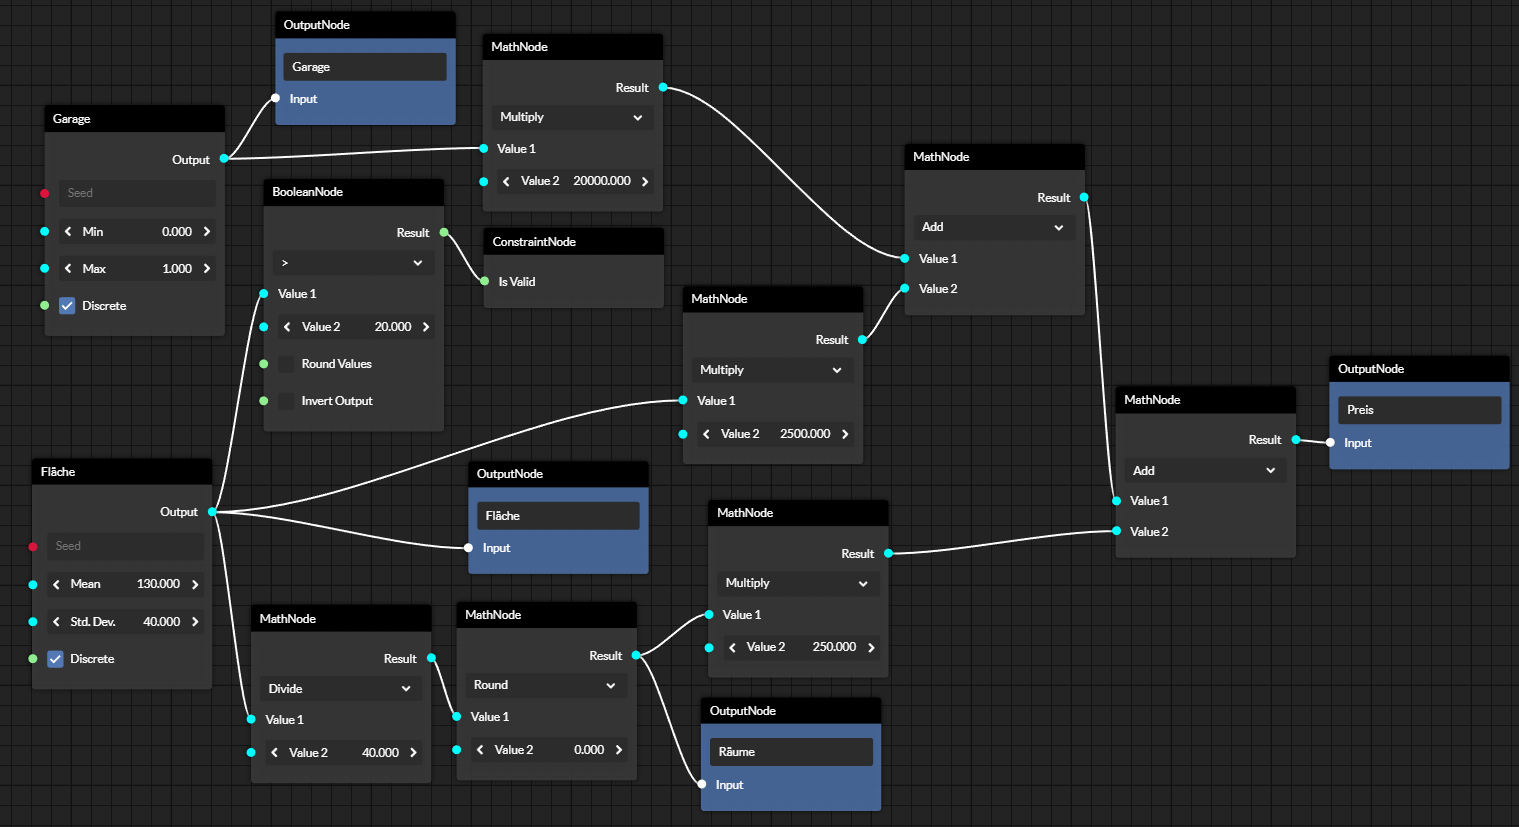
\includegraphics[width=1\textwidth]{usertestsolution.PNG}
    \caption{Musterlösung der Aufgabe}
    \label{fig:vuereactivity}
\end{figure}

\subsection{Resultate auswerten}

\subsubsection{Zeit, die für das Lösen der Aufgabe benötigt wird}
Die Aufgabe konnte von allen Versuchspersonen innerhalb von 30 - 45 Minuten gelöst werden. Diese Zeit beinhaltet nur das Lösen der Aufgabe an sich, nicht das Lesen der Anleitung und Aufgabe oder das anschließende Gespräch. Im Durchschnitt haben die Versuchspersonen damit etwas länger gebraucht als die erwarteten 30 Minuten.

\subsubsection{Zufriedenheit der Versuchspersonen bezüglich Usability}
Das Konzept von \ac{DFP} haben alle Versuchsteilnehmern innerhalb weniger Minuten verstanden. Im Verlauf des Tests kamen allerdings bei allen Versuchsteilnehmern ähnliche Probleme bezüglich der Usability auf:
\begin{itemize}
    \item Teile des Kontextmenüs im Editor sind außerhalb des Bildschirms wenn das Kontextmenü zu nah am Rand geöffnet wird
    \item Es war zuerst unklar, dass sich der Wert einer Eingangsschnittstelle direkt über das dazugehörige Steuerelement verändern lässt, wenn die Schnittstelle nicht verbunden ist
    \item Viele der Versuchsteilnehmer haben rausgezoomed um einen besseren Überblick über den Gesamtgraphen zu haben. Dadurch wurde es schwierig, beim Verbinden die Verbindungspunkte der Knoten-Schnittstellen zu treffen.
    \item Die Scrollbar beim Dropdown-Menü für die Operation des Mathematikknotens ist kaum sichtbar. Dadurch musste der Versuchsleiter oft einen Tipp geben, dass der Mathematikknoten noch deutlich mehr Operationen enthält als direkt angezeigt werden.
    \item Das automatische Konvertieren von Datentypen (wie zum Beispiel von Boolean, also true/false, nach Number, also 0/1) ist weder direkt ersichtlich noch in der Anleitung beschrieben. Auch hier musste bei allen Versuchsteilnehmern ein Tipp vom Versuchsleiter gegeben werden.
    \item Beim Umbenennen von Knoten muss der Name innerhalb der Textbox erst markiert werden. Dabei darf allerdings die Maus nicht außerhalb der Textbox losgelassen werden, da dies den Prozess den Umbennens beendet und die Textbox ausblendet. Des Weiteren wurde von einigen Probanden gewünscht, dass auch bei angepassten Name der Typ des Knotens weiterhin ersichtlich bleibt.
\end{itemize}

\subsubsection{Häufigkeit der Inanspruchnahme von Hilfe des Versuchsleiters}
Alle Versuchsteilnehmer haben in etwa gleich viele Tipps bekommen. Konkret gab der Versuchsleiter pro Versuch etwa 5 - 10 Tipps. Meistens zielten die Tipps darauf ab, den Probanden Zeit zu sparen, damit der Versuch sich nicht zu sehr in die Länge zieht.

\subsubsection{Unerwartete Schwierigkeiten der Versuchspersonen bei der Durchführung eines konkreten Teils der Aufgabe}
Alle Teilnehmer hatten Probleme damit, bei der Berechnung des Preises 20000 Euro zu addieren, wenn die Wohnung eine Garage hat. Dies kam zum einen durch das vorher beschriebene Problem, dass die Versuchspersonen nicht wussten, dass Datentypen wie Boolean automatisch zu einer Nummer konvertiert werden können. Im Gespräch mit den Probanden kam aber heraus, dass viele eine Art \enquote{Switch}-Knoten vermisst haben. Dieser sollte eine Boolean-Eingangsschnittstelle, zwei Eingangsschnittstellen ohne Typ und eine Ausgangsschnittstelle ohne Typ haben. Liegt an der Boolean-Eingangsschnittstelle der Wert \texttt{false} an, hat die Ausgangsschnittstelle den Wert der ersten Eingangsschnittstelle ohne Typ, liegt der Wert \texttt{true} an, hat sie den Wert der zweiten Eingangsschnittstelle ohne Typ.

\subsubsection{Allgemeine Erkenntnisse}
Zusätzlich zu den bereits genannten Ergebnissen konnten durch die Beobachtung der Versuchspersonen weitere Erkenntnisse gewonnen werden:
\begin{itemize}
    \item Es hat sich als schwierig herausgestellt, einen guten Anfang zu finden. Dies hängt mit Sicherheit damit zusammen, dass die Versuchspersonen das Tool zum ersten Mal benutzt haben. Hierfür wäre es sinnvoll, eine Art Tutorial oder Einführung zu haben, bei der ein kleines Beispielmodell aufgebaut wird. Dies könnte beispielsweise als Video umgesetzt werden und würde für neue Nutzer sehr hilfreich sein.
    \item Die Versuchspersonen gingen beim Aufbau des Modells sehr unterschiedlich vor. Im Prinzip lassen sich die Vorgehensweisen in zwei Kategorien einteilen. Zum einen gab es die \enquote{Debugger}. Diese nutzten temporäre Ausgabeknoten und die \textit{Preview Data} Funktion, um sich Zwischenergebnisse anzeigen zu lassen. Das Modell wurde Stück für Stück aufgebaut und immer wieder überprüft, ob der Fortschritt korrekt ist. Auf der anderen Seite gab es diejenigen, die das Modell komplett aufbauten, bevor sie überhaupt auf die Daten schauen. Durch Tipps vom Versuchsleiter kam es dabei zu keinen Fehlern. Die Tipps wurden gegeben, damit die Probanden im späteren Verlauf des Versuchs keine zeitaufwändige Fehlersuche durchführen müssen. Gerade bei größeren Modellen ist zu erwarten, dass die Fehlerquote bei der zweiten Vorgehensweise sehr hoch ist. Aus diesem Grund sollte das Debugging vereinfacht und gefördert werden. Beispielsweise könnte eine Funktion im Kontextmenü eines Knotens hinzugefügt werden, die es erlaubt, die im aktuellen Graphen entstehenden Werte der Ausgabeschnittstellen des Knotens in einem Popup-Fenster einzusehen.
\end{itemize}